\documentclass{beamer}
%[envcountsect]

\usepackage{multicol, multirow, enumerate}
\usepackage{lmodern}
\usepackage[english]{babel}
\usepackage{pgf}
%\usepackage{pgf,pgfarrows,pgfnodes,pgfautomata,pgfheaps}
\usepackage{graphics, amsfonts, dsfont, graphicx, animate, epsfig}
\usepackage{color, xcolor, colortbl}
\usepackage{amsmath, amssymb, amsthm}
\usepackage[latin1]{inputenc}
\setbeamertemplate{theorems}[numbered]
\usepackage{times}
\usepackage{tikz}
\usepackage{verbatim}
\usetikzlibrary{arrows,shapes}
\usepackage{bbding}
\usepackage{array}
\usepackage{tkz-euclide}
\usepackage{gensymb}
\usepackage{hyperref, bm, etoolbox, mathtools}
\usepackage{mathrsfs}
\usetikzlibrary{calc,intersections}
\definecolor{bblue}{RGB}{163,187,221}
\definecolor{rred}{RGB}{238,147,153}

\newcommand{\defn}{\triangleq}
\newcommand{\Bern}{\textnormal{Bern}}
\newcommand{\Unif}{\textnormal{Unif}}
\newcommand{\Normal}{\textnormal{N}}
\newcommand{\logNormal}{\textnormal{LN}}
\newcommand{\Bin}{\textnormal{Bin}}
\newcommand{\NB}{\textnormal{NB}}
\newcommand{\HG}{\textnormal{HG}}
\newcommand{\Geom}{\textnormal{Geom}}
\newcommand{\Beta }{\textnormal{Beta}}
\newcommand{\BetaBin}{\textnormal{Beta-Bin}}
\newcommand{\Ga}{\textnormal{Ga}}
\newcommand{\Exp}{\textnormal{Exp}}
\newcommand{\Expo}{\textnormal{Expo}}
\newcommand{\Po}{\textnormal{Po}}
\newcommand{\Multi}{\textnormal{Multi}}
\newcommand{\student}{\textnormal{t}}
\newcommand{\Cauchy}{\textnormal{Cauchy}}
\newcommand{\Pareto}{\textnormal{Pareto}}
\newcommand{\Laplace}{\textnormal{Laplace}}
\newcommand{\Logistic}{\textnormal{Logistic}}
\newcommand{\Dir}{\textnormal{Dir}}
\newcommand{\DP}{\textnormal{DP}}
\newcommand{\Inv}{\textnormal{Inv-}}

\newcommand{\pa}{\partial}
\newcommand{\RV}{\textsc{rv}}
\newcommand{\cdf}{\textsc{cdf}}
\newcommand{\cgf}{\textsc{cgf}}
\newcommand{\pdf}{\textsc{pdf}}
\newcommand{\pmf}{\textsc{pmf}}
\newcommand{\chf}{\textsc{chf}}
\newcommand{\mgf}{\textsc{mgf}}
\newcommand{\EF}{\textsc{EF}}
\newcommand{\NEF}{\textsc{NEF}}
\newcommand{\MLE}{\textsc{mle}}
\newcommand{\MAP}{\textsc{MAP}}
\newcommand{\Med}{\textsc{Med}}
\newcommand{\MME}{\textsc{mme}}
\newcommand{\QME}{\textsc{qme}}
\newcommand{\UMVUE}{\textsc{umvue}}
\newcommand{\MPT}{\textsc{MPT}}
\newcommand{\UMPT}{\textsc{UMPT}}
\newcommand{\LRT}{\textsc{LRT}}


\newcommand{\simiid}{\stackrel{iid}{\sim}}
\newcommand{\ind}{\mathds{1}}
\newcommand{\pr}{\mathbb{P}}
\newcommand{\E}{\mathbb{E}}
\newcommand{\Var}{\mathbb{V}ar}
%%% ### Algebraic Operators
%%%----------------------------------------------------------------------------%%%
\newcommand{\sn}{\sum_{i=1}^n}
\newcommand{\pn}{\prod_{i=1}^n}
\newcommand{\f}[2]{\frac{#1}{#2}}
\newcommand{\bo}[1]{\boldsymbol{#1}}
\newcommand{\sto}[1]{\sum_{i=1}^{#1}}
\newcommand{\sft}[2]{\sum_{i=#1}^{#2}}
\newcommand{\fn}[1]{{\footnotesize #1}}
%%%----------------------------------------------------------------------------%%%
%%% ### Limit Operators
%%%----------------------------------------------------------------------------%%%
\newcommand{\limn}{\lim_{n\to\infty}}
\newcommand{\limh}{\lim_{h\to0}}
%%% ### Math Set Notation
%%%----------------------------------------------------------------------------%%%
\newcommand{\Q}{\mathbb{Q}}
\newcommand{\Z}{\mathbb{Z}}
\newcommand{\R}{\mathbb{R}}
\newcommand{\C}{\mathbb{C}}
\newcommand{\N}{\mathbb{N}}
\newcommand{\F}{\mathscr{F}}
\newcommand{\el}{\mathscr{L}}
\newcommand{\sol}[1]{{\color{blue}{\textbf{Solution:} #1}}}
\newcommand{\dis}[1]{{\displaystyle #1}}
\newcommand{\vs}[1]{\vspace{#1 cm}}
\newcommand{\wwt}{\frac{\partial}{\partial \theta}}

\newenvironment{mymathbox}
{\par\smallskip\centering\begin{lrbox}{0}%
\begin{minipage}[c]{0.95\textwidth}}
{\end{minipage}\end{lrbox}%
\framebox[0.98\textwidth]{\usebox{0}}%
\par\medskip
\ignorespacesafterend}

\newcommand{\rotateRPY}[3]% roll, pitch, yaw
{   \pgfmathsetmacro{\rollangle}{#1}
    \pgfmathsetmacro{\pitchangle}{#2}
    \pgfmathsetmacro{\yawangle}{#3}

    % to what vector is the x unit vector transformed, and which 2D vector is this?
    \pgfmathsetmacro{\newxx}{cos(\yawangle)*cos(\pitchangle)}
    \pgfmathsetmacro{\newxy}{sin(\yawangle)*ffcos(\pitchangle)}
    \pgfmathsetmacro{\newxz}{-sin(\pitchangle)}
    \path (\newxx,\newxy,\newxz);
    \pgfgetlastxy{\nxx}{\nxy};

    % to what vector is the y unit vector transformed, and which 2D vector is this?
    \pgfmathsetmacro{\newyx}{cos(\yawangle)*sin(\pitchangle)*sin(\rollangle)-sin(\yawangle)*cos(\rollangle)}
    \pgfmathsetmacro{\newyy}{sin(\yawangle)*sin(\pitchangle)*sin(\rollangle)+ cos(\yawangle)*cos(\rollangle)}
    \pgfmathsetmacro{\newyz}{cos(\pitchangle)*sin(\rollangle)}
    \path (\newyx,\newyy,\newyz);
    \pgfgetlastxy{\nyx}{\nyy};

    % to what vector is the z unit vector transformed, and which 2D vector is this?
    \pgfmathsetmacro{\newzx}{cos(\yawangle)*sin(\pitchangle)*cos(\rollangle)+ sin(\yawangle)*sin(\rollangle)}
    \pgfmathsetmacro{\newzy}{sin(\yawangle)*sin(\pitchangle)*cos(\rollangle)-cos(\yawangle)*sin(\rollangle)}
    \pgfmathsetmacro{\newzz}{cos(\pitchangle)*cos(\rollangle)}
    \path (\newzx,\newzy,\newzz);
    \pgfgetlastxy{\nzx}{\nzy};
}

\tikzset{RPY/.style={x={(\nxx,\nxy)},y={(\nyx,\nyy)},z={(\nzx,\nzy)}}}


\mode<presentation> {

  %\usetheme{Warsaw}
  %\usetheme{Pittsburgh}
  %\usetheme{Montpellier}
  \usetheme{Madrid}
  %\usetheme{Hannover}
  %\usetheme{default}
  %\usetheme{CambridgeUS}
  %\usecolortheme{dolphin,crane}

  \setbeamercovered{transparent}
    \framebreak
  %\allowdisplaybreaks
  \usefonttheme[onlymath]{serif}
  }


\title[Causal Isotonic Regression]{Causal Isotonic Regression}
\subtitle{}
\author[Billy, Heman, Martin]{Billy, Heman, Martin}
\date{Summer, 2020}

 \AtBeginSubsection[] {
  \begin{frame}<beamer>
    \frametitle{Agenda}
    \tableofcontents[currentsection,currentsubsection]
  \end{frame}
}

\begin{document}
% \usebackgroundtemplate{\includegraphics[width=\paperwidth,height=\paperheight]{JSM}}
% \setbeamerfont{supertitle}{size=\LARGE,parent=structure}
% \def\supertitle#1{\gdef\@supertitle{#1}}%

%%%%%%%%%%%%%%%%%%%%%%%%%%%%%%%%%%%%%%%%%%%%%%%%%%

\begin{frame}
\vspace{2cm}
\hfill
    \begin{beamercolorbox}[wd=0.95\paperwidth,ht=7ex,dp=3.8ex,center]{title}
      \usebeamerfont{supertitle}\@ {\Large Reading Group: Causal Isotonic Regression}
    \end{beamercolorbox}
\textcolor{blue}{\textbf{\begin{large}
\\
\vspace{0.5cm}
\begin{center}
{\large Ted Westling, Peter Gilbert, Marco Carone (JRSSB, 2020)}
\end{center}
\end{large}}}
\vspace{0.5cm}
\end{frame}

\usebackgroundtemplate{...}

\AtBeginSection{
\begin{frame}
\frametitle{Agenda}
\tableofcontents[currentsection]
\end{frame}
}

%%%%%%%%%%%%%%%%%%%%%%%%%%%%%%%%%%%%%%%%%%%%%%%%%%     P.2
\section{Introduction}
%\section{Motivation and Literature Review}
%%%%%%%%%%%%%%%%%%%%%%%%%%%%%%%%%%%%%%%%%%%%%%%%%%     P.3

\begin{frame}{Terminologies}
There are some common terminologies to be introduced.
\begin{block}{Terminoloies}
	\begin{enumerate}
		\item \textbf{Observational Studies:} Conduct inference based on the data set we observed, i.e. we did not make any control on the experiment.

		\item \textbf{Experimental Design:} Randomly assigning the values of the exposure and observe the corresponding response.

		\item \textbf{Association:} $X$ is positively associated with $Y$ iff $X$ increases together with $Y$.

		\item \textbf{Causation:} Increase in $X$ results in increase in $Y$.
	\end{enumerate}
\end{block}
In general, we cannot draw causation conclusion under framework of observation studies due to the existence of confounders.\\
\textbf{AIM 1:} Accessing causality effect by using observational data set.
\end{frame}

\begin{frame}{Literature Review}
	\begin{enumerate}
		\item Non-parametric methods with \textbf{binary/categorical exposure}
		\begin{enumerate}
			\item Inverse-probability-weighted estimators\\ \textit{(Horvitz and Thompson, 1952)}

			\item Augmented inverse-probability-weighted (AIPW) estimators \textit{(Scharfstein et al., 1999; Bang and Robins, 2005)}

			\item Targeted minimum-loss-based estimators \\
			\textit{(van der Laan and Rose, 2011)}
		\end{enumerate}

	    \item \textbf{Continuous exposure}\\
	    Common approach: Discretize the continuous interval into two or more region and apply above methods under categorial case.

	\end{enumerate}
	\textit{Remark:} Undesirable method as we are commonly interested in the causal dose response curver, which describes the causal relationship between the exposure and outcome across a \textbf{continuum} of the exposure
\end{frame}

\begin{frame}{Literature Review}
We further consider existing method dealing with continuous exposures.
	\begin{enumerate}
		\item Applying parametric models \textit{(Robins, 2000 and Zhang et al., 2016)}

		\item Inference on parameters obtained by projecting a causal dose-response curve onto a parametric working model. \textit{(Neugebauer and van der Laan, 2007)}

		\item nonparametric	estimation using flexible data-adaptive algorithms\\
		\textit{(Rubin and van der Laan, 2006 and Diaz and van der Laan, 2011)}

		\item estimator based on local linear smoothing
		\textit{(Kennedy et al, 2017)}

		\item general framework for inference on parameters that fail to be sufficiently smooth as a function of the data-generating distribution and for which regular root-n-estimation theory is therefore not available.
		\textit{(van der Laan et al., 2018)}
	\end{enumerate}

\end{frame}

\begin{frame}{Comment on existing methodologies}
	For the literature on non-parametric estimation of causal dose-response curves, the large sample inference is not valid and is sensitive to selection of certain tuning parameters.\\
	Smoothing-based methods are sensitive to choice of kernel function and bandwidth. The estimators commonly have non-negligible bias.

\end{frame}

\begin{frame}{Motivation for isotonic regression}
   In many setting, the causal dose-response curve is a monotone function For example, exposures such as daily exercise performed, cigarettes smoked per week
   and air pollutant levels are all known to have monotone relationships with various health outcomes.\\
   Recall in the setting of linear regression, we are interested in estimating the function $g$ s.t.
   $$
   \E(Y|X_1,\cdots,X_p)=g(X_1,\cdots,X_p).
   $$
   For linear regression, we assumed linearity on the model, i.e. restrict the class of estimating cuver for $g$ to class of the linear function $\E(Y|X_1,\cdots,X_p)=g(X_1,\cdots,X_p)=\beta_0+\beta_1 X_1+\cdots+\beta_pX_p$ for some $\beta_0,\beta_1,\cdots,\beta_p$. However, linearity is usually too strong as the model assumption. In contrast, we add only trivial restriction on the class of function under non-parametric function for estimation $g$.
\end{frame}

\begin{frame}{Motivation for isotonic regression}
	However, as mentioned, the estimator in non-parametric methods might be easily affected by choice of kernel and bandwidth. And as an intermediate level of assumption, we may assume $g$ to be a monotone function. Notice that linearity implies monotonicity but the converse does not holds. The regression with monotonicity assumption is known as \textbf{Isotonic Regression}.\\
	The following are some advantages of isotonic regression
	\begin{enumerate}
		\item Does not require linearity assumption.
		\item Does not require selection of kernel and bandwidth.
		\item Invariance to strictly increasing transformation of exposure and on centring and scaling by factor of $n^{-1/3}$.
	\end{enumerate}
    If there is not confounding variables, we can directly estimate the causal isotonic curve. However as mentioned, the authur attempted access causality under confounded setting in this paper.
\end{frame}


%\section{Parameter of interest and causal interpretation}

\begin{frame}{Notation}
	\begin{enumerate}
		\item $Y$: Response.
		\item $A$: Continuous exposure.
		\item $W$: Vector of covariates.
		\item $O\defn (Y,A,W)$: Data unit.
		\item $P_0$: The true data-generating distribution
		\item $\mathcal{O}=\mathcal{Y}\times \mathcal{A}\times\mathcal{W}$: Support of $P_0$, where $\mathcal{Y},\mathcal{A}\subseteq \R$ are intervals and $\mathcal{W}\subseteq \R^p$.
	\end{enumerate}
\end{frame}

\begin{frame}{Parameter of interest}
	Denote $E_0$ as the expectation under the law $P_0$. Our parameter of interest, known as \textbf{G-computed regression function} from $\mathcal{A}$ to $\E$ is defined as
	$$
	a\mapsto \theta_0(a)\defn \E_0\big\{\E_0(Y|A=a,W) \big\}
	$$
	, which has causation interpretation in some scientific contexts. It kind of measure the \textbf{effect of $A$ on $Y$ after accounted for $W$}.
\end{frame}

\begin{frame}{Causal parameter and unadjusted regression function}
Adopting the idea of randomnized experiment, for each fixed $a\in\mathcal{A}$, we denote by $Y(a)$ the potential outcome (i.e. a R.V.) under exposure level $A=a$. The causal parameter is thus defined as $m_0:\mathcal{A}\to\R$ through
$$
m_0(a)\defn \E_0\big\{Y(a)\big\}
$$
annd the resulting curve is known as \textbf{\textit{causal dose-response curve}}.\\
We can also denote the \textbf{unadjusted} regression function as $r_0(a)\defn\E_0(Y|A=a)$, which is the standard quantity of interest in regression analysis.\\
Under different set of conditions, we can claim that $m_0(a)=r_0(a)$ and $m_0(a)=\theta_0(a)$, meaning that those causal conditions allows us to draw causation conclusion from observational data set.
\end{frame}

\begin{frame}{Comparison among quantities}
\begin{enumerate}
	\item Causal dose-response curve: $m_0(a)\defn \E_0\big\{Y(a)\big\}$ measures the intrinsic casual effect of $A$ on $Y$.
	\item G computed regression function: $\theta_0(a)\defn \E_0\big\{\E_0(Y|A=a,W) \big\}$ measures the effect of $A$ on $Y$ after accounted for covariates $W$
	\item Unadjusted regression function: $r_0(a)\defn\E_0(Y|A=a)$ measures the association between $A$ on $Y$
\end{enumerate}
Therefore, the strength of causation statement can be made through these functions are different. Even though we may not be able to contain all covariates in $W$, it gives more informative conclusion than only relying on $r_0(a)$.
\end{frame}

\begin{frame}{Causal condition: $m_0(a)=r_0(a)$}
\begin{block}{Causal condition 1}
	Suppose that for some $a\in \mathcal{A}$,
	\begin{enumerate}
		\item Each unit's potential outcomes are independent of all other units' exposures.

		\item $Y=Y(A)$, where $Y$ is the response and $Y(A)$ is defined as in setting of randomnized experiment.

		\item $A$ and $Y(a)$ are independent.

		\item The marginal density of $A$ is positive at $a$.
	\end{enumerate}
    then for such $a\in \mathcal{A}$, we have $m_0(a)=r_0(a)$, i.e. the causal effect for exposure level $A=a$.
\end{block}
\textit{
Remark:
} Condition (3) is commonly only satisfied in randomnized trials as usually ther exist some confounders affecting both $A$ and $Y(a)$, which induce dependency.
\end{frame}


\begin{frame}{Causal condition: $m_0(a)=\theta_0(a)$}
Condition (3) and (4) are being too strong to be practical, it is natural to find sufficient condition s.t. inference of $\theta_0(a)$ give meaningful result.
	\begin{block}{Causal condition 2}
		Suppose that for some $a\in \mathcal{A}$,
		\begin{enumerate}
			\item Each unit's potential outcomes are independent of all other units' exposures.

			\item $Y=Y(A)$, where $Y$ is the response and $Y(A)$ is defined as in setting of randomnized experiment.

			\item $A$ and $Y(a)$ are \textbf{conditionally} independent given $W$.

			\item The marginal density of $A$ \textbf{given} $\bo{W}$ is a.s. positive at $a$
		\end{enumerate}
		then for such $a\in \mathcal{A}$, we have $m_0(a)=\theta_0(a)$, i.e. the causal effect for exposure level $A=a$.
	\end{block}
	\textit{
		Remark:
	} Whenever $m_0(a)=\theta_0(a)$, the conclusion drawn from inference can be interpreted as causal statement.
\end{frame}

%\section{Contribution and organization of the paper}
\begin{frame}{Notations}
	\begin{enumerate}
		\item $F_P:\mathcal{A}\to\R$ the distribution function of $A$ under $P$.

		\item $\F_\theta:$ class of non-decreasing real-valued functions on $\mathcal{A}$.

		\item $\F_T$: class of strictly increasing and continuous distribution functions supported on $\mathcal{A}$.
	\end{enumerate}
	The statistical model to work on is given by
	$$
	\mathcal{M}\defn \big\{
	P:\theta_P\in\F_\theta,F_P\in\F_T
	\big\}
	$$
	Recall our target: Making inference about $$\theta_0(a)=\E_0\big\{E_0(Y|A=a,W) \big\}$$ for cts exposure $A$ and monotone $\theta_0$ by using \textbf{independent} (NOT randomnized) observations $O_1,\cdots,O_n$ drawn from $P_0\in\mathcal{M}$, which is an extension of classical isotonic regression in sense of allowing the existence of confounders.
\end{frame}

\begin{frame}{Contribution of paper}
\begin{block}{Contributions}
	\fn{
\begin{enumerate}
	\item generalizes the unadjusted isotonic regression estimator to the more realistic scenario in which there is confounding by recorded covariates.

	\item investigate finite sample and asymptotic properties of the estimator proposed, including invariance to strictly increasing transformations of the exposure, doubly robust consistency	and doubly robust convergence in distribution to a non-degenerate limit.

	\item derive practical methods for constructing pointwise confidence intervals, including intervals that have valid doubly robust calibration.

	\item illustrate numerically the practical performance of the estimator.
\end{enumerate}
}
\end{block}
\end{frame}

%%%%%%%%%%%%%%%%%%%%%%%%%%%%%%%%%%%%%%%%%%%%%%%%%%
\section{Proposed approach}
%%%%%%%%%%%%%%%%%%%%%%%%%%%%%%%%%%%%%%%%%%%%%%%%%%

\begin{frame}{Classical least square isotonic regression}
  Linear regression: find $\beta=\hat{\beta}$ s.t. $\sn \big( Y_i -\beta A_i \big)^2$ is minimized \\
  Isotonic regression: find $r=r_n$ s.t. $\sn \big[ Y_i -r(A_i) \big]^2$ is minimized
  \begin{itemize}
    \item $Y_{1:n}$: responses
    \item $A_{1:n}$: continuous exposures
    \item $r$: any monotone non-decreasing function
    \item $r_n$ can be obtained via pool adjacent violators algorithm (PAVA)
    \begin{itemize}
      \item Not true without assuming piecewise linearity of $r$?
      \item PAVA can be used to find best monotone fit $\hat{Y}_i$ only
    \end{itemize}
    \item $r_n$ can also be represented by greatest convex minorants (GCMs)
    \begin{itemize}
      \item Probably because isotonic regression can be formulated as a convex programming problem
      \item See section 2.3 of the R package \href{https://cran.r-project.org/web/packages/isotone/vignettes/isotone.pdf}{\textit{isotone}'s vignette}
    \end{itemize}
  \end{itemize}
\end{frame}

\begin{frame}{Pool adjacent violators algorithm}
  \animategraphics[scale=0.4, alttext=graphical illustration of PAVA]{10}{Causal Isotonic Regression/pava-}{0}{40} \\
  \fn{Source: \href{http://fa.bianp.net/blog/2013/isotonic-regression/}{Pedregosa, Fabian (2013)}}
\end{frame}

\begin{frame}{Pool adjacent violators algorithm}
  Target: find best monotone fit $\hat{Y}_i$ of response $Y_i$
  \begin{itemize}
    \item Exposure $A_i$ are ordered in $i$ first, i.e. $A_1 \le A_2 \le \dots \le A_n$
    \item Response $Y_i$ may not be monotone as the sorting is done on $A_i$
    \item Fit $\hat{Y}_i = r_n(A_i)$ must be monotone in $i$
    \begin{itemize}
      \item That's why $r=r_n$ should be a monotone non-decreasing function
      \item Identifiable without assuming piecewise linearity of $r$?
    \end{itemize}
  \end{itemize}
  Algorithm (sketch):
  \begin{enumerate}
    \item Initialize $l:=0$, $B^{(0)}:=n$, $\hat{Y}_r^{(0)} := Y_r$ for $r=1, \dots, n$
    \item Merge $\hat{Y}^{(l)}$-values into blocks if $\hat{Y}_{r+1}^{(l)} < \hat{Y}_r^{(l)}$ for $r=1, \dots, B^{(l)}$
    \item Minimize the loss function for each block $r$, which gives $\hat{Y}_r^{(l+1)}$
    \item If $\hat{Y}_{r+1}^{(l)} < \hat{Y}_r^{(l)}$ for some $r$, set $l = l+1$ and go back to step 2
    \item Expand the block values w.r.t. to $i=1, \dots, n$
  \end{enumerate}
\end{frame}

\begin{frame}{Greatest convex minorant}
  GCM of a function $f$ bounded on $[a,b]$: supremum over all convex functions $g$ such that $g \le f$ \\
  \vs{0.5}
  Let $F_n$ be the empirical distribution function of $A_{1:n}$. It can be shown that the isotonic regression estimator $r_n(a)$ is
  \begin{itemize}
    \item the left derivative, evaluated at $F_n(a)$,
    \item of the GCM over the interval $[0,1]$ of the linear interpolation,
    \item of the cumulative sum diagram $\left\{ \f{1}{n} \left[ i, \sum_{j=0}^i Y_{(i)}^* \right]: i=0,1,\dots,n \right\}$,
    \item where $Y_{(0)}^* := 0$ and $Y_{(i)}^*$ is the response $Y$ sorted by value of exposure $A$
  \end{itemize}
\end{frame}

\begin{frame}{Attractive properties of isotonic regression estimator}
  No need to choose kernel, bandwidth or any other tuning parameter
  \begin{itemize}
    \item The monotone fit restriction is kind of like a kernel already
    \item but it is true that no choice of tuning parameter is needed
  \end{itemize}
  Invariant to strictly increasing transformations of $A$ \\
  \vs{0.1}
  Uniform consistency on any strict subinterval of $A$ \\
  \vs{0.1}
  Limit distribution available
  \begin{itemize}
    \item $n^{\f{1}{3}} \big[r_n(a) -r_0(a) \big] \stackrel{d}{\rightarrow} \big[ 4r'_0(a) \sigma_0^2(a)/f_0(a) \big]^{\f{1}{3}} \mathbb{W}$
    for any interior point $a \in \mathcal{A}$ at which $r'_0(a)$, $f_0(a) := F'_0(a)$ and $\sigma_0^2(a) := E_0 \big[ \{ Y -r_0(a) \}^2 |A=a \big]$ exist and are positive and continuous in a neighbourhood of $a$
    \item $\mathbb{W}$ follows Chernoff's distribution, which often appears in the limit distribution of monotonicity-constrained estimators
  \end{itemize}
\end{frame}

\begin{frame}{Definition of proposed estimator}
  \begin{block}{Definition: pointwise outcome}
    $$\mu_P(a,w) := E_P(Y|A=a,W=w)$$ for any given $P \in \mathcal{M}$
  \end{block}
  \begin{block}{Definition: normalized exposure density}
    $$g_P(a,w) := \pi_P(a|w)/f_P(a)$$
    where $\pi_P(a|w)$ is the conditional density evaluated at $a$ given $W=w$, $f_P$ is the marginal density of $A$ under $P$
  \end{block}
  \begin{block}{Definition: pseudo-outcome}
    $$\xi_{\mu,g,Q}(y,a,w) := \f{y-\mu(a,w)}{g(a,w)} +\int \mu(a,z) Q(dz)$$
  \end{block}
\end{frame}

\begin{frame}{Monotonicity of proposed estimator} \label{slide:monotonicity}
  Kennedy \textit{et al.} (2017) used pseudo-outcome to develop local linear regression for inference of $\theta_0(a)$. In the setting of this paper, $\theta_0(a)$ is known to be monotone
  \begin{itemize}
    \item I think the monotonicity of $\theta_0(a)$ is an assumption
    \item Yet it seems reasonable as continuous treatment usually has monotone causal effect (if effective) within certain range
    \item Example: daily exercise time (0-2 hours) on life expectancy
    \item Counterexample: daily exercise time (0-12 hours)
    \item So the reasonability of monotonicity may depend on the range of treatment $A$ (experiemental) or data exploration (observational)
  \end{itemize}
  Under monotonicity, it is natural to consider the isotonic regression of the pseudo-outcomes on $A_{1:n}$
\end{frame}

\begin{frame}{Proposed estimation procedure} \label{slide:procedure}
  \begin{block}{Estimation of $\theta_n(a)$}
    \begin{enumerate}
      \item Construct estimators $\mu_n, g_n$ of $\mu_0, g_0$ respectively
      \item For each $a$ in the unique values of $A_{1:n}$, compute and set
      \begin{align}
        \textstyle \Gamma_n(a) &:= \textstyle \f{1}{n} \sn I_{(-\infty,a]}(A_i) \f{Y_i -\mu_n(A_i,W_i)}{g_n(A_i,W_i)} \nonumber \\
          &\quad \textstyle +\f{1}{n^2} \sn \sum_{j=1}^n I_{(-\infty,a]}(A_i) \mu_n(A_i,W_j) \label{eq:GammaN}
      \end{align}
      \item Compute the GCM $\bar{\Psi}_n$ of the set of points $\{(0,0)\} \cup \{\big( F_n(A_i), \Gamma_n(A_i) \big): i=1,2,\dots,n \}$ over $[0,1]$
      \item Define $\theta_n(a)$ as the left derivative of $\bar{\Psi}_n$ evaluated at $F_n(a)$
    \end{enumerate}
  \end{block}
\end{frame}

\begin{frame}{Asymptotic framework for the proposed estimator}
  As in Kennedy \textit{et al.} (2017), $\theta_n(a)$ deviate from classical results \\
  \begin{itemize}
    \item Pseudo-outcomes $\xi_{\mu,g,Q}(y,a,w)$ are dependent because they depend on the estimator $\mu_n, g_n, Q_n$ estimated with all observations
    \item Hence classical results from isotonic regression do not apply
    \item However, $\theta_n$ is of generalized Grenander type
    \item Asymptotic results of Westling and Carone (2020) can be used
  \end{itemize}
  We skip the proof of $\theta_n$ to be Grenander type here, which is to show $\theta_n$ falls in the class of estimator discussed in Westling and Carone (2020)
\end{frame}

\begin{frame}{Some remarks on monotonicity and generality} \label{slide:generality}
  Monotonicity: if $\theta_0(a)$ were only known to be monotone on a fixed subinterval $\mathcal{A}_0 \subset \mathcal{A}$
  \begin{itemize}
    \item We discuss this assumption on page \ref{slide:monotonicity}
    \item The estimation procedure is still valid by first defining $F_p(a):=P(A \le a| A \in \mathcal{A}_0)$ and $F_n$ as its empirical counterpart
    \item Then replace $I_{(-\infty,a]}(A_i)$ in equation \ref{eq:GammaN} by $I_{(-\infty,a] \cap \mathcal{A}_0}(A_i)$
  \end{itemize}
  Generality: the proposed estimator $\theta_n$ generalizes the classical $r_n$
  \begin{itemize}
    \item Condition 1: $A \perp \!\!\! \perp W \implies g_0(a,w) = 1$, so we may take $g_n=1$
    \item Condition 2: $Y|A \perp \!\!\! \perp W|A \implies \mu_n(a,w)=\mu_n(a)$
    \item Under these conditions, equation \ref{eq:GammaN} becomes
    $$\Gamma_n(a) = \f{1}{n} \sn I_{(-\infty,a]}(A_i) Y_i -\mu_n(A_i)$$
    \item As a result, $\theta_n(a) = r_n(a)$ for each $a$
  \end{itemize}
\end{frame}

%%%%%%%%%%%%%%%%%%%%%%%%%%%%%%%%%%%%%%%%%%%%%%%%%%
\section{Theoretical properties}
%%%%%%%%%%%%%%%%%%%%%%%%%%%%%%%%%%%%%%%%%%%%%%%%%%

\begin{frame}{Invariance to strictly increasing transform of exposure}
  $\theta_n(a)$ is invariant to strictly increasing transform $H(\cdot)$ of exposure $A$
  \begin{itemize}
    \item Intuition: composition preserve monotonicity
    \item Desirable property since scale of exposure is often arbitrary
    \item Example: temperature in degrees Fahrenheit or Celsius or in kelvins
    \item Change of scale does not affect available information
  \end{itemize}
  We skip the proof because the intuition is simple (composition of monotone functions is also monotone)
\end{frame}

\begin{frame}{Condtions for consistency}
  Notations:
  \begin{itemize}
    \item $\mathcal{F}$: a uniformly bounded class of functions
    \item $Q$: a finite discrete probability measure
    \item $N\{ \epsilon, \mathcal{F}, L_2(Q) \}$: the $\epsilon$-covering-number, i.e. the smallest number of $L_2(Q)$ balls of radius less than or equal to $\epsilon$ needed to cover $\mathcal{F}$
    \item $\log\big[ \sup_Q N\{ \epsilon, \mathcal{F}, L_2(Q) \} \big]$: the uniform $\epsilon$-entropy of $\mathcal{F}$
  \end{itemize}
  \begin{block}{Condition 1}
    There exist constants $C, \delta, K_0, K_1, K_2 \in (0, \infty)$ and $V \in [0,2)$ s.t., almost surely as $n \rightarrow \infty$, $\mu_n$ and $g_n$ are contained in classes of functions $\mathcal{F}_0$ and $\mathcal{F}_1$ respectively, satisfying
    \begin{enumerate}
      \item $|\mu| \le K_0, \forall \mu \in \mathcal{F}_0$, and $K_1 \le g \le K_2, \forall g \in \mathcal{F}_1$
      \item $\log\big[ \sup_Q N\{ \epsilon, \mathcal{F}_0, L_2(Q) \} \big] \le C \epsilon^{-V/2}$ and $\log\big[ \sup_Q N\{ \epsilon, \mathcal{F}_1, L_2(Q) \} \big] \le C \epsilon^{-V}, \forall \epsilon \le \delta$
    \end{enumerate}
  \end{block}
\end{frame}

\begin{frame}{Condtions for consistency}
  $P_0$: the true data-generating distribution but not projection
  \begin{block}{Condition 2}
    There exists $\mu_\infty \in \mathcal{F}_0$ and $g_\infty \in \mathcal{F}_1$ s.t. $P_0(\mu_n -\mu_\infty)^2 \stackrel{p}{\rightarrow} 0$ and $P_0(g_n -g_\infty)^2 \stackrel{p}{\rightarrow} 0$
  \end{block}
  \begin{block}{Condition 3}
    There exist subsets $\mathcal{S}_1, \mathcal{S}_2, \mathcal{S}_3$ of $\mathcal{A} \times \mathcal{W}$ s.t. $P_0(\mathcal{S}_1 \cup \mathcal{S}_2 \cup \mathcal{S}_3)=1$ and
    \begin{enumerate}
      \item $\mu_\infty(a,w) = \mu_0(a,w), \forall (a,w) \in \mathcal{S}_1$
      \item $g_\infty(a,w) = g_0(a,w), \forall (a,w) \in \mathcal{S}_2$
      \item $\mu_\infty(a,w) = \mu_0(a,w)$ and $g_\infty(a,w) = g_0(a,w), \forall (a,w) \in \mathcal{S}_3$
    \end{enumerate}
  \end{block}
  These conditions control the uniform entropy of certain classes of functions, which is related to empirical process theory. A thorough treatment is provided in van der Vaart and Wellner (1996)
\end{frame}

\begin{frame}{Consistency}
  \begin{block}{Theorem 1}
    If Conditions 1-3 hold, then $\theta_n(a) \stackrel{p}{\rightarrow} \theta_0(a)$ for any value $a \in \mathcal{A}$ s.t. $F_0(a) \in (0,1)$, $\theta_0$ is continuous at $a$ and $F_0$ is strictly increasing in a neighbourhood of $a$. \\
    \vs{0.3}
    If $\theta_0$ is uniformly continuous and $F_0$ is strictly increasing on $\mathcal{A}$, then $\sup_{a \in \mathcal{A}_0} \big[ \theta_n(a) -\theta_0(a) \big] \stackrel{p} 0$ for any bounded strict subinterval $\mathcal{A}_0 \subset \mathcal{A}$.
  \end{block}
  (Well-known) boundary issues with Grenander-type estimators:
  \begin{itemize}
    \item In the pointwise statement, $F_0(a)$ is required to be in $[0,1]$
    \item Similarly, the uniform statement only covers strict subintervals of $\mathcal{A}$
    \item Various remedies have been proposed before to mitigate this
    \item Potential direction for future research
  \end{itemize}
\end{frame}

\begin{frame}{Remark on Condtions for consistency} \label{slide:remarkCon1}
  \begin{block}{Remark on Condition 1}
    Condition 1 requires that $\mu_n$ and $g_n$ eventually be contained in uniformly bounded function classes that are sufficiently small for certain empirical process terms to be controlled.
    This is satisfied by parametric classes and many infinite dimensional function classes. See chapter 2.6 of van der Vaart and Wellner (1996). \\
    \vs{0.3}
    There is also an asymmetry between the entropy requirements for $\mathcal{F}_0$ and $\mathcal{F}_1$ in part 2 of Condition 1. This is due to the term $\int \int_{-\infty}^a \mu_n(u,w) F_n(du) Q_n(dw)$ appearing in $\Gamma_n(a)$.
    To control this term, an upper bound of the form $\int_0^1 \log\big[ \sup_Q N\{ \epsilon, \mathcal{F}_0, L_2(Q) \} \big] d\epsilon$ from the theory of empirical $U$-process is used (Nolan and Pollard, 1987). \\
    \vs{0.3}
    The later part of this paper (section 3.7) considers the use of cross-fitting to avoid these entropy conditions in Condition 1.
  \end{block}
\end{frame}

\begin{frame}{Remark on Condtions for consistency} \label{slide:remarkCon3}
  \begin{block}{Remark on Condition 2 and 3}
    Condition 2 requires that $\mu_n$ and $g_n$ tend to limit functions $\mu_\infty$ and $g_\infty$, and Condition 3 requires that requires that either $\mu_\infty(a,w) = \mu_0(a,w)$ or $g_\infty(a,w) = g_0(a,w)$ for $(F_0 \times Q_0)$ almost every $(a,w)$.
    \begin{itemize}
      \item This is equivalent to saying that $\mu_n$ or $g_n$ is consistent?
      \item Seems to be in line with Kennedy \textit{et al.} (2017)
    \end{itemize}
    If either
    \begin{enumerate}
      \item $\mathcal{S}_1$ and $\mathcal{S}_3$ are null sets or
      \item $\mathcal{S}_2$ and $\mathcal{S}_3$ are null sets,
    \end{enumerate}
    then Condition 3 is known simply as double robustness of the estimator $\theta_n$ relative to the nuisance functions $\mu_0$ and $g_0$: $\theta_n$ is consistent as long as $\mu_\infty = \mu_0$ or $g_\infty = g_0$.
    However, Condition 3 is more general than classical double robustness as at least one of $\mu_n$ or $g_n$ tends to the truth for \textbf{only} almost every point in the domain.
  \end{block}
\end{frame}

\begin{frame}{Double robustness} \label{slide:doubleRobust}
  Multiply robustness: preserve consistency even if a subset of the $N$ nuisance models is mispecified in the procedure \\
  Double robustness: $N=2$, so one model can be mispecified \\
  \begin{block}{Example: inverse probability weighted (IPW) estimator}
    \begin{itemize}
      \item $Y_i$: response; $A_i \in \{0,1\}$: treatment; $W$: covariates
      \item Estimator: $\hat{\mu}^{i-IPW} = \f{1}{n} \sn \f{A_i Y_i}{\pi_0(W_i)}$ where $\pi_0(W) = P(A=1|W)$
      \begin{itemize}
        \item Often infeasible since functional form $\pi_0(W)$ is unknown
        \item (Example) nuisance model 1: $\pi_0(W) = \pi(W; \alpha_0) = \f{\exp(\alpha_0^T \tilde{W})}{1 +\exp(\alpha_0^T \tilde{W})}$
        \item $\hat{\mu}^{f-IPW} = \f{1}{n} \sn \f{A_i Y_i}{\pi(W_i; \hat{\alpha})}$
      \end{itemize}
      \item Augmented IPW (AIPW) estimator:
      \begin{itemize}
        \item $\hat{\mu}^{f-\phi-IPW} = \f{1}{n} \sn \left[ \f{A_i Y_i}{\pi(W_i; \hat{\alpha})} +\left\{ 1 -\f{A_i}{\pi(W_i; \hat{\alpha})} \right\} \phi(W_i) \right]$
        \item Nuisance model 2: $\phi(W)=E(Y|W,A=1)$ is the most efficient
      \end{itemize}
    \end{itemize}
  \end{block}
  See \href{https://statnav.files.wordpress.com/2017/10/doublerobustness-preprint.pdf}{Daniel (2017)} for a simple introduction to this topic
\end{frame}

\begin{frame}{Conditions for convergence in distribution}
  Notations:
  \begin{itemize}
    \item $d(h_1,h_2; a,\epsilon,\mathcal{S})$: pseudodistance; $\sigma_0^2(a,w)$: conditional variance
    \item $d(h_1,h_2; a,\epsilon,\mathcal{S}) := \scriptstyle \sqrt{\sup_{|u-a| \le \epsilon} E_0 \big[ I_\mathcal{S}(u,W) \{ h_1 u,W) -h_2(u,W) \}^2 \big]}$
    \item $\sigma_0^2(a,w) := E_0 \big[ \{Y -\mu_0(A,W)\}^2 | A=a, W=w \big]$
  \end{itemize}
  \begin{block}{Condition 4}
    There exists $\epsilon_0 > 0$ s.t.
    \begin{enumerate}
      \item $\max \big[ d(\mu_n,\mu_\infty; a,\epsilon_0,\mathcal{S}_1), d(g_n,g_\infty; a,\epsilon_0,\mathcal{S}_2) \big] = o_p(n^{-1/3})$
      \item $\max \big[ d(\mu_n,\mu_\infty; a,\epsilon_0,\mathcal{S}_2), d(g_n,g_\infty; a,\epsilon_0,\mathcal{S}_1) \big] = o_p(1)$
      \item $d(\mu_n,\mu_\infty; a,\epsilon_0,\mathcal{S}_3) d(g_n,g_\infty; a,\epsilon_0,\mathcal{S}_3) = o_p(n^{-1/3})$
    \end{enumerate}
  \end{block}
  \begin{block}{Condition 5}
    $F_0, \mu_0, \mu_\infty, g_0, g_\infty$ and $\sigma_0^2$ are continuously differentiable in a neighbourhood of $a$ uniformly over $w \in \mathcal{W}$
  \end{block}
\end{frame}

\begin{frame}{Convergence in distribution}
  \begin{block}{Theorem 2}
    If Conditions 1-5 hold, then
    $$
      n^{1/3} \{ \theta_n(a) -\theta_0(a) \} \stackrel{d}{\rightarrow} \left\{ \f{4 \theta'_0(a) \kappa_0(a)}{f_0(a)} \right\}^{1/3} \mathbb{W}
    $$
    for any $a \in \mathcal{A}$ such that $F_0(a) \in (0,1)$, where $\mathbb{W}$ follows the standard Chernoff distribution and
    $$
      \kappa_0(a) := \scriptstyle E_0 \left( E_0\left[ \left\{ \f{Y-\mu_\infty(a,W)}{g_\infty(a,W)} +\theta_\infty(a) -\theta_0(a) \right\}^2 \Big| A=a,W \right] g_0(a,W) \right)
    $$
    with $\theta_\infty(a)$ denoting $\int \mu_\infty(a,w) Q_0(dw)$.
  \end{block}
  We skip the comparison between the limit distributions of $\theta_n$ and $r_n$ as it is paritally discussed in p.\ref{slide:generality}. In short, their limit distributions only differ in concentration, which is analogous to findings in linear regression
\end{frame}

\begin{frame}{Remark on Conditions for convergence in distribution}
  \begin{block}{Remark on Condition 4 and 5}
    The requirements of Condition 4 is equivalent to
    \begin{enumerate}
      \item On $\mathcal{S}_1$ where $\mu_n$ is consistent but $g_n$ is not, $\mu_n$ converges faster than $n^{-1/3}$ uniformly in a neighbourhood of $a$,
      \item Similarly for $g_n$ on $\mathcal{S}_2$ and
      \item On $\mathcal{S}_3$ where both $\mu_n$ and $g_n$ are consistent, only the product of their rates of convergence must be faster than $n^{-1/3}$
    \end{enumerate}
    This suggests the possibility of performing doubly robust inference for $\theta_0(a)$, which is explored in section 4.
    Note that as discussed in p.\ref{slide:remarkCon3}, these conditions are more general than the classical double robustness
  \end{block}
  We skip the discussion of plug-in estimator $\theta_{\mu_n}(a)$, which can achieve faster rate of convergence than $\theta_n(a)$ but hinges entirely on the consistency of $\mu_n$ and may not admit a tractable limit theory
\end{frame}

\begin{frame}{Grenander-type estimation without domain transform}
  The proposed estimator $\theta_n(a)$ coincides with a generalized Grenander-type estimator for which the marginal exposure empirical distribution function is used as domain transformation \\
  \vs{0.3}
  An alternative estimator $\bar{\theta}_n$ could be constructed via Grenander-type estimation \textbf{without} the use of any domain transformation. We skip its construction here but there are several points to note:
  \begin{itemize}
    \item $\bar{\theta}_n$ does not generalize the classical isotonic regression
    \item $\bar{\theta}_n$ is not invariant to strictly increasing transform of $A$
    \item Domain of $\mathcal{A}$ needs to be known/chosen in defining $\bar{\theta}_n$
    \item When $\mu_\infty = \mu_0$, $\theta_n(a)$ and $\bar{\theta}_n$ may have the same limit distribution
    \item When $\mu_\infty \neq \mu_0$, $\bar{\theta}_n$ is dominated by $\theta_n(a)$ in AMSE sense
    \begin{itemize}
      \item The transformation improves statistical efficiency in this case
      \item Relative gain in efficiency is directly related to the asymptotic bias
    \end{itemize}
  \end{itemize}
\end{frame}

\begin{frame}{Discrete domains}
  When $A$ is discrete, $\theta_n(a)$ is asymptotically equivalent to the AIPW estimator, which is paritally discussed in p.\ref{slide:doubleRobust} \\
  \vs{0.5}
  As a result, the large sample properties of $\theta_n(a)$ can be derived from the large sample properties of the AIPW estimator and asymptotically valid inference can be obtained by using standard influence-function-based techniques \\
  \vs{0.5}
  We skip the proof here as it is like realizing the isotonic regression of pseudo-outcome under discrete exposure coincides with the AIPW estimator. Instead, we shall have a short discussion on influence function
\end{frame}

\begin{frame}{Influence function}
  \begin{block}{Definition of influence function (Hampel \textit{et al.}, 1986)}
    Let $T(F)$ be a statistical functional where $F$ is a distribution. The influence function of $T$ at $F$ is given by
    $$IF(x;T,F) := \lim_{t \downarrow 0} \f{T\big[ (1-t)F +t \delta_x \big] -T(F)}{t}$$
    in those $x \in \mathcal{X}$ where this limit exists.
  \end{block}
  A complete discussion of this definition usually requires G\^{a}teaux differentiability. We cover some of its usage instead:
  \begin{itemize}
    \item An estimator $\hat{\theta} \approx \theta(P_0) +E_n\big[ IF(X) \big]$ can be dominated by a single outlier \textbf{unless} $IF$ is bounded
    \item Asymptotic efficiency bound (Bias, Variance)
    \item Distributional decomposition, partial identification etc.
  \end{itemize}
  See \href{https://scholar.harvard.edu/files/kasy/files/ifhandout.pdf}{this note} for a quick summary
\end{frame}

\begin{frame}{Large sample results for causal effects}
  The result so far concerns about the causal dose-response $a \mapsto m_0(a)$, which may not hold for the causal effect $(a_1, a_2) \mapsto m_0(a_1) -m_0(a_2)$ \\
  \vs{0.3}
  If the identification conditions discussed in Section 1.2 applied to each of $a_1$ and $a_2$, such causal effects can be identified with the observed data parameter $\theta_0(a_1) -\theta_0(a_2)$ \\
  \vs{0.3}
  If the condtions of Theorem 1 hold for both $a_1$ and $a_2$, we can establish consistency via the use of continuous mapping theorem \\
  \vs{0.3}
  However, Theorem 2 only provides marginal distributional results. Joint convergence result is thus required for inference of causal effect
\end{frame}

\begin{frame}{(Joint) convergence for causal effects}
  \begin{block}{Theorem 3}
    Define $Z_n(a_1,a_2) := \left( n^{1/3} \big\{ \theta_n(a_1) -\theta_0(a_1) \big\}, n^{1/3} \big\{ \theta_n(a_2) -\theta_0(a_2) \big\} \right)$. If Conditions 1-5 hold for $a \in \{a_1, a_2\} \subset \mathcal{A}$ and $F_0(a_1), F_0(a_2) \in (0,1)$, then
    $$
      Z_n(a_1,a_2) \stackrel{d}{\rightarrow}
      \left( \big\{ 4 \tau_0(a_1) \big\}^{1/3} \mathbb{W}_1, \big\{ 4 \tau_0(a_2) \big\}^{1/3} \mathbb{W}_2 \right)
    $$
    where $\mathbb{W}_1, \mathbb{W}_2$ are independent standard Chernoff distributions and the scale parameter $\tau_0 = \f{\theta'_0(a) \kappa_0(a)}{f_0(a)}$ is as defined in theorem 2.
  \end{block}
  Note that Theorem 3 implies
  $$
    \scriptstyle n^{1/3} \left[ \big\{ \theta_n(a_1) -\theta_n(a_2) \big\} -\big\{ \theta_0(a_1) -\theta_0(a_2) \big\} \right] \stackrel{d}{\rightarrow}
    \scriptstyle \big\{ 4 \tau_0(a_1) \big\}^{1/3} \mathbb{W}_1 -\big\{ 4 \tau_0(a_2) \big\}^{1/3} \mathbb{W}_2
  $$
\end{frame}

\begin{frame}{Cross-fitting to avoid empirical process conditions}
  In observational studies, researchers can rarely specify a \textit{priori} correct parametric models for $\mu_0$ and $g_0$.
  This motivates use of data-adaptive estimators to meet Conditions 2 and 3 \\
  \vs{0.3}
  However, such estimators often leads to violation of Condition 1, or it may be onerous to determine that they do not. See slide p.\ref{slide:remarkCon1} \\
  \vs{0.3}
  In the context of asymptotically linear estimators, it has been noted that cross-fitting nuisance estimators can resolve this challenge by eliminating empirical process conditions \\
  \vs{0.3}
  Therefore, this paper proposes cross-fitting of $\mu_n$ and $g_n$ to avoid entropy conditions in Theorem 1 and 2
\end{frame}

\begin{frame}{Estimation with cross-fitting}
  \begin{block}{Estimation procedure with cross-fitting}
    \begin{enumerate}
      \item Fix $V \in \{ 2,3,\dots,n/2 \}$
      \item Randomly partition the indices $\{ 1,2,\dots,n \}$ into $V$ sets $\mathcal{V}_{n,1},\mathcal{V}_{n,2},\dots,\mathcal{V}_{n,V}$
      \item Assume $N := n/V \in \Z^+$. For each $v \in \{ 1,2,\dots,V \}$:
      \begin{enumerate}
        \item Define $\mathcal{T}_{n,v} := \{ O_i: i\notin \mathcal{V}_{n,v} \}$ as the \textit{training set} for fold $v$
        \item Construct $\mu_{n,v}$ and $g_{n,v}$ using only observations from $\mathcal{T}_{n,v}$
      \end{enumerate}
      \item Define pointwise the cross-fitted estimator $\Gamma_n^\circ$ of $\Gamma_0$ as
      $\begin{aligned}
        \textstyle \Gamma_n^\circ(a) &:= \textstyle \f{1}{V} \sum_{v=1}^V \Big[ \f{1}{N} \sum_{i \in \mathcal{V}_{n,v}} I_{(-\infty,a]}(A_i) \f{Y_i -\mu_{n,v}(A_i,W_i)}{g_{n,v}(A_i,W_i)} \\
        &\quad \textstyle + \f{1}{N^2} \sum_{i,j \in \mathcal{V}_{n,v}} I_{(-\infty,a]}(A_i) \mu_{n,v}(A_i,W_j) \Big]
      \end{aligned}$
      \item Construct the cross-fitted estimator $\theta_n^\circ$ as in p.\ref{slide:procedure}
    \end{enumerate}
  \end{block}
  Remark: all results hold as long as $\max_v n/|\mathcal{V}_{n,v}| = O_p(1)$
\end{frame}

\begin{frame}{Conditions for convergence under cross-fitting}
  \begin{block}{Condition 6}
    There exist constants $C',\delta',K'_0,K'_1,K'_2,K'_3 \in (0,\infty)$ s.t., almost surely as $n \rightarrow \infty$ and for all $v$, $\mu_{n,v}$ and $g_{n,v}$ are contained in classes of functions $\mathcal{F}'_0$ and $\mathcal{F}'_1$ respectively, satisfying
    \begin{enumerate}
      \item $|\mu| \le K'_0, \forall \mu \in \mathcal{F}'_0$, and $K'_1 \le g \le K'_2, \forall g \in \mathcal{F}'_1$, and
      \item $\sigma_0^2(a,w) \le K'_3$ for almost all $a$ and $w$
    \end{enumerate}
  \end{block}
  \begin{block}{Condition 7}
    There exist $\mu_\infty \in \mathcal{F}'_0$ and $g_\infty \in \mathcal{F}'_1$ s.t. $\max_v P_0(\mu_{n,v} -\mu_\infty)^2 \stackrel{p}{\rightarrow} 0$ and $\max_v P_0(g_{n,v} -g_\infty)^2 \stackrel{p}{\rightarrow} 0$
  \end{block}
\end{frame}

\begin{frame}{Conditions for convergence under cross-fitting}
  \begin{block}{Condition 8}
    There exists $\epsilon_0 > 0$ s.t.
    \begin{enumerate}
      \item $\max \big[ d(\mu_{n,v},\mu_\infty; a,\epsilon_0,\mathcal{S}_1), d(g_{n,v},g_\infty; a,\epsilon_0,\mathcal{S}_2) \big] = o_p(n^{-1/3})$
      \item $\max \big[ d(\mu_{n,v},\mu_\infty; a,\epsilon_0,\mathcal{S}_2), d(g_{n,v},g_\infty; a,\epsilon_0,\mathcal{S}_1) \big] = o_p(1)$
      \item $d(\mu_{n,v},\mu_\infty; a,\epsilon_0,\mathcal{S}_3) d(g_{n,v},g_\infty; a,\epsilon_0,\mathcal{S}_3) = o_p(n^{-1/3})$
    \end{enumerate}
  \end{block}
  Remark: Conditions 6, 7 and 8 are analogue of Conditions 1, 2 and 4 respectively under cross-fitting
\end{frame}

\begin{frame}{Convergence under cross-fitting}
  \begin{block}{Theorem 4}
    If Conditions 6, 7 and 3 hold, then $\theta_n^\circ(a) \stackrel{p}{\rightarrow} \theta_0(a)$ for any value $a \in \mathcal{A}$ s.t. $F_0(a) \in (0,1)$, $\theta_0$ is continuous at $a$ and $F_0$ is strictly increasing in a neighbourhood of $a$. \\
    \vs{0.3}
    If $\theta_0$ is uniformly continuous and $F_0$ is strictly increasing on $\mathcal{A}$, then $\sup_{a \in \mathcal{A}_0} \big[ \theta_n^\circ(a) -\theta_0(a) \big] \stackrel{p} 0$ for any bounded strict subinterval $\mathcal{A}_0 \subset \mathcal{A}$.
  \end{block}
  \begin{block}{Theorem 5}
    If Conditions 6, 7, 3, 8, 5 hold, then
    $$
      n^{1/3} \{ \theta_n^\circ(a) -\theta_0(a) \} \stackrel{d}{\rightarrow} \left\{ 4 \tau_0(a) \right\}^{1/3} \mathbb{W}
    $$
    for any $a \in \mathcal{A}$ such that $F_0(a) \in (0,1)$, where $\mathbb{W}$ follows the standard Chernoff distribution.
  \end{block}
\end{frame}

%%%%%%%%%%%%%%%%%%%%%%%%%%%%%%%%%%%%%%%%%%%%%%%%%%
%%%%%%%%%%%%%%%%%%%%%%%%%%%%%%%%%%%%%%%%%%%%%%%%%%
\section{Construction of confidence intervals}
%%%%%%%%%%%%%%%%%%%%%%%%%%%%%%%%%%%%%%%%%%%%%%%%%%
%%%%%%%%%%%%%%%%%%%%%%%%%%%%%%%%%%%%%%%%%%%%%%%%%%

%%%%%%%%%%%%%%%%%%%%%%%%%%%%%%%%%%%%%%%%%%%%%%%%%%
%% Section 4.1
%%%%%%%%%%%%%%%%%%%%%%%%%%%%%%%%%%%%%%%%%%%%%%%%%%

%%%%%%%%%%%%%%%%%%%%%%%%%%%%%%%%%%%%%%%%%%%%%%%%%% p.1

\begin{frame}{Wald-type Confidence Interval}

\begin{block}{Wald-type CI}
	Since the limit distribution of $n^{1/3} \Big[ \theta_n(a)-\theta_0(a) \Big]$ is symmetric around zero by the result of Theorem 2, writing $\tau_0(a):=\theta^{'}_0(a)\kappa_0(a)/f_0(a)$ and denoting by $\tau_n(a)$ any consistent estimator of $\tau_0(a)$ , then a Wald-type $1-\alpha$ level asymptotic confidence interval for $\theta_0(a)$ is given by
	\begin{center}
	$\Big[ \theta_n(a)-\Big[ \frac{4\tau_n(a)}{n} \Big]^{1/3} \ q_{1-\alpha /2}, \ \theta_n(a)+\Big[ \frac{4\tau_n(a)}{n} \Big]^{1/3} \ q_{1-\alpha /2}  \Bigg] $,
	\end{center}
	where $q_p$ denotes the $p^{th}$ quantile of $\mathbb{W}$.
\end{block}

\end{frame}

%%%%%%%%%%%%%%%%%%%%%%%%%%%%%%%%%%%%%%%%%%%%%%%%%% p.2

\begin{frame}{Wald-type Confidence Interval}

\begin{block}{Estimation of $\tau_0(a)$}
  Since estimation of $\tau_0(a)$ involves, it can be estimated either direcly or indirectly, estimation of $\theta^{'}_0(a)/f_0(a)$ and $\kappa_0(a)$.
  For direct estimation, we note that $\theta^{'}_0(a)/f_0(a)=\psi^{'}_0(F_0(a))$ with $\psi_0:=\theta_0 \circ F^{-1}_0$.It suggests that
  	\begin{enumerate}
  	\item Estimate $\theta^{'}_0$ and $f_0$ separately and consider the ratio of these of estimators; or
  	\item Estimate $\psi^{'}_0$ directly and compose it with the estimator of $F_0$.
  	\end{enumerate}

  For indirect estimation, it involves the invariance property of the scale estimator to strictly monotone transformations of the exposure. To estimate $\psi^{'}_0$, we recall that the estimator $\psi_n$ from Section 2 is a step function and is not differentiable. A Natural Solution consists of computing the derivative of a smoothed version of $\psi_n$. We have found local quadratic kernel smoothing of points $\lbrace (u_j,\psi_n(u_j)):j=1,2,\cdots,\rbrace$, for $u_j$ the midpoints of the jump points of $\psi_n$, to work well in practice.
\end{block}

\end{frame}

%%%%%%%%%%%%%%%%%%%%%%%%%%%%%%%%%%%%%%%%%%%%%%%%%% p.3

\begin{frame}{Wald-type Confidence Interval}

\begin{block}{Wald-type CIs for causal effects}
	Theorem 3 is used to construct the Wald-type CIs for causal effects in the form $\theta_0(a_1)-\theta_0(a_2)$, then a Wald-type $1-\alpha$ level asymptotic confidence interval for $\theta_0(a_1)-\theta_0(a_2)$ is given by
	\begin{center}
	$\Big[ \theta_n(a_1)-\theta_n(a_2) - \bar{q}_{n,1-\alpha/2}n^{-1/3}, \ \theta_n(a_1)-\theta_n(a_2) + \bar{q}_{n,1-\alpha/2}n^{-1/3} \Bigg] $
	\end{center}
	where $\bar{q}_{n,1-\alpha/2}$ denotes the $(1-\alpha/2)$ quantile of $\big[4\tau_n(a_1)\big]^{1/3} \mathbb{W}_1 - \big[4\tau_n(a_2)\big]^{1/3} \mathbb{W}_2$, $\mathbb{W}_1$ and $\mathbb{W}_2$ are independent Chernoff distributions, using Monte Carlo simulations.
\end{block}

\end{frame}

%%%%%%%%%%%%%%%%%%%%%%%%%%%%%%%%%%%%%%%%%%%%%%%%%%
%% Section 4.2
%%%%%%%%%%%%%%%%%%%%%%%%%%%%%%%%%%%%%%%%%%%%%%%%%%

%%%%%%%%%%%%%%%%%%%%%%%%%%%%%%%%%%%%%%%%%%%%%%%%%% p.4

\begin{frame}{Scale estimation relying on consistent nuisance estimation}

\begin{block}{Plug-in estimator of $\kappa_0(a)$}
	Consider settings in which both $\mu_n$ and $g_n$ are consistent estimators. In such cases, we have $\kappa_0(a)=E_0\big[ \sigma_0^2(a,W)/g_0(a,W)\big]$ with $\sigma^2_0(a,W)$ denoting the conditional variance $E_0\lbrace  \big[ Y - \mu_0(a,W) \big]^2 | A=a,W=w \rbrace$. Then, a plug-in estimator of $\kappa_0(a)$ is given by
	\begin{center}
	$\kappa_n(a):=\frac{1}{n}\sn \frac{\sigma_n^2(a,W_i)}{g_n(a,W_i)}$
	\end{center}
	 Any regression technique could be used to estimate the conditional expectation of $Z_n:= \big[ Y - \mu_(a,W) \big]^2$ given A and W. If $\mu_n$, $g_n$ and $\sigma_n^2$ are consistent estimator, then $\kappa_n(a)$ is a consistent estimator.
\end{block}

\end{frame}


%%%%%%%%%%%%%%%%%%%%%%%%%%%%%%%%%%%%%%%%%%%%%%%%%%
%% Section 4.3
%%%%%%%%%%%%%%%%%%%%%%%%%%%%%%%%%%%%%%%%%%%%%%%%%%

%%%%%%%%%%%%%%%%%%%%%%%%%%%%%%%%%%%%%%%%%%%%%%%%%% p.5

\begin{frame}{Doubly-robust scale estimation}
	Aim: To construct an estimator of $\kappa_0(a)$ consistent even of either $\mu_{\infty} \neq \mu_0$ or $g_{\infty} \neq g_0$
\begin{block}{Doubly-robust estimator of $\kappa_0(a)$}
	Note that $\kappa_0(a)=lim_{h\downarrow 0} E_0 \big[ K_h (F_0(A)-F_0(a)) \eta_{\infty}(Y,A,W) \big]$, where $K_h:u \mapsto h^{-1} K(uh^{-1})$ for some bounded density function K with bounded support, and defined
	\begin{center}
	$\eta_{\infty}:(y,a,w)\mapsto \Bigg[ \frac{y-\mu_{\infty}(a,w)}{g_{\infty}(a,w)} + \theta_{\infty}(a) - \theta_0(a)\Bigg]^2$
	\end{center}
	Setting $\theta_{\mu_n}(a):= \int \mu_n(a,w)Q_n(dw)$ with $Q_n$ the empirical distribution based on $W_1,W_2,\cdots,W_n$, and define
	\begin{center}
	$\kappa^{*}_{n,h}(a)=\frac{1}{n} \sn  K_h (F_n(A_i)-F_n(a)) \eta_{n}(Y_i,A_i,W_i)$
	\end{center}
	by substituting $\mu_{\infty},g_{\infty},\theta_{{\infty}},\theta_0$ by $\mu_n,g_n,\theta_{\mu_n},\theta_n$.
\end{block}

\end{frame}

%%%%%%%%%%%%%%%%%%%%%%%%%%%%%%%%%%%%%%%%%%%%%%%%%% p.6

\begin{frame}{Doubly-robust scale estimation}

\begin{block}{Doubly-robust estimator of $\kappa_0(a)$(Con'd)}
	Under conditions (A1)-(A5), it can be shown that $\kappa^{*}_{n,h_n}(a) \stackrel{P}{\rightarrow} \kappa_0(a)$ by standard kernel smoothing arguments for any sequence $h_n \rightarrow 0$. In particular, $\kappa^{*}_{n,h_n}(a)$ is consistent under the general form of doubly-robustness specified by condition(A3).

\end{block}

\begin{block}{Appropriate value of bandwidth h}
	We propose the following empirical criterion:
	\begin{enumerate}
	\item Define the integrated scale $\gamma_0:=\int\kappa_0(a)F_0(da)$ and construct the estimator $\gamma_n(h):=\int\kappa_{n,h}(a)F_n(da)$ for any candidate $h>0$.
	\item Observe that $\gamma_0=E_0[\eta_{\infty}(Y,A,W)]$, which suggest $\bar{\eta}_n:=\frac{1}{n} \sn \eta_n(Y_i,A_i,W_i)$.
	\end{enumerate}
	It motivates us to define $h^{*}_n:=argmin_h [\gamma_n(h)-\bar{\eta_n}]^2$.
\end{block}

The proposed doubly-robust estimator of $\kappa_0(a)$ is $\kappa_{n,DR}(a):=\kappa_{n,h_n^{*}}(a)$.

\end{frame}

%%%%%%%%%%%%%%%%%%%%%%%%%%%%%%%%%%%%%%%%%%%%%%%%%% p.7

\begin{frame}{Doubly-robust scale estimation}

\begin{block}{Remarks}
	\begin{enumerate}
	\item	$\kappa_{n,DR}(a)$ only depends on A and a through the ranks $F_n(A)$ and $F_n(a)$. Hence, the estimator is invariant to strictly monotone transformations of the exposure.
	\item If $\mu_n(a,w)=\mu_n(a)$ does not depend on $w$ and $g_n=1$, $\kappa_{n,DR}(a)$ tends to the conditional variance $Var_0(Y|A=a)$, which is precisely the scale parameter appearing in standard isotonic regression.
	\end{enumerate}
\end{block}

\end{frame}

%%%%%%%%%%%%%%%%%%%%%%%%%%%%%%%%%%%%%%%%%%%%%%%%%%
%% Section 4.4
%%%%%%%%%%%%%%%%%%%%%%%%%%%%%%%%%%%%%%%%%%%%%%%%%%

%%%%%%%%%%%%%%%%%%%%%%%%%%%%%%%%%%%%%%%%%%%%%%%%%% p.8

\begin{frame}{Confidence intervals via sample splitting}

	Sample splitting method recently proposed by Banerjee er al.(2019) could also be used to perform inference. To implement the approach in our context: (1)we randomly split the sample into $m$ subsets of roughly equal size;(2) perform the estimation procedure on each subset to form subset-specific estimates $\theta_{n,1},\theta_{n,2},\cdots,\theta_{n,m}$; and (3) define $\bar{\theta}_{n,m}(a):=\frac{1}{m}\sum^m_{j=1}\theta_{n,j}(a)$.
	 If $m>1$ is fixed, then under mild conditions $\bar{\theta}_{n,m}(a)$ has strictly better asymptotic MSE than $\theta_n(a)$.

\begin{block}{CI via sample splitting}
	For moderate m, the asymptotic $1-\alpha$ level confidence interval for $\theta_0(a)$ is given by
	\begin{center}
	$\Bigg[ \bar{\theta}_{n,m}(a)-\frac{\sigma_{n,m}(a)}{\sqrt{m}n^{1/3}}t_{1-\alpha/2,m-1}, \ \bar{\theta}_{n,m}(a)+\frac{\sigma_{n,m}(a)}{\sqrt{m}n^{1/3}}t_{1-\alpha/2,m-1} \Bigg]$
	\end{center}
	where $\sigma^2_{n,m}(a):=\frac{1}{m-1} \sum^m_{j=1}[\theta_{n,j}(a)-\bar{\theta}_{n,m}(a)]^2$ and $t_{1-\alpha/2,m-1}$ is the $(1-\alpha/2)$ quantile of the t-distribution with $m-1$ degrees of freedom.
\end{block}

\end{frame}

%%%%%%%%%%%%%%%%%%%%%%%%%%%%%%%%%%%%%%%%%%%%%%%%%%
%%%%%%%%%%%%%%%%%%%%%%%%%%%%%%%%%%%%%%%%%%%%%%%%%%
\section{Numerical studies}
%%%%%%%%%%%%%%%%%%%%%%%%%%%%%%%%%%%%%%%%%%%%%%%%%%
%%%%%%%%%%%%%%%%%%%%%%%%%%%%%%%%%%%%%%%%%%%%%%%%%%

%%%%%%%%%%%%%%%%%%%%%%%%%%%%%%%%%%%%%%%%%%%%%%%%%% p.9

\begin{frame}{Numerical Studies}

	Goals: Perform numerical experiments to assess the performance of the proposed estimators of $\theta_0(a)$ and of the three approaches for constructing confidence intervals, which we also compare to that of
the local linear estimator and associated confidence intervals proposed in Kennedy et al.(2017).

\begin{block}{Idea of Data Generating Process}
	\begin{enumerate}
	\item	Generate $W \in \R^4$ as a vector of four independent standard normal variate.
	\item	Generate $U$ given $W$, and then transform $U$ to obtain $A$. ($\because$ the estimation procedures requires estimating the conditional density of $U:=F_0(A)$ given $W$)
	\end{enumerate}

\end{block}

\end{frame}

%%%%%%%%%%%%%%%%%%%%%%%%%%%%%%%%%%%%%%%%%%%%%%%%%% p.10

\begin{frame}{Data Generating Process}

	\begin{enumerate}
	\item	$W \sim N(0,\sum)$
	\\where $\sum$ is the $4\times4$ diagonal matrix with value 1.
	\item		$U \sim \bar{g}_0(u|w)=I_{[0,1]}(u)\lbrace \lambda(w) + 2u[1-\lambda(w)]\rbrace$
	\\where $\lambda(w):=0.1+1.8 \ expit(\beta^{\top}w).$
	\item	$A \sim 0.5N(-2,1)+0.5N(2,1)$
	\item	$[Y|A=a,W=w] \sim Bern(\mu_0(a,w))$
	\\where $\mu_0(a,w):=expit(\gamma^{\top}_1 \underline{w} + \gamma^{\top}_2 \underline{w}a + \gamma_3 a^2)$
	\item $\beta = (-1,-1,1,1)^{\top}, \gamma_1 = (-1,-1,-1,1,1)^{\top}, \gamma_1 = (3,-1,-1,1,1)^{\top}$ and $\gamma_3=3$
	\end{enumerate}

\end{frame}

%%%%%%%%%%%%%%%%%%%%%%%%%%%%%%%%%%%%%%%%%%%%%%%%%% p.11

\begin{frame}{Estimation and Conditions}

\begin{block}{Estimator used}
	\begin{enumerate}
	\item	Causal isotonic regression estimator $\theta_n$.
	\item	Local linear estimator of Kennedy et al.(2017) with data-driven bandwidth selection procedure proposed in Section 3.5.
	\item	Sample-splitting version of $\theta_n$ with $m=5$ splits.
	\end{enumerate}
\end{block}

\begin{block}{Settings}
	\begin{enumerate}
	\item Both $\mu_n$ and $g_n$ are consistent.
	\item Only $\mu_n$ is consistent.
	\item Only $g_n$ is consistent.
	\end{enumerate}
\end{block}

\end{frame}

%%%%%%%%%%%%%%%%%%%%%%%%%%%%%%%%%%%%%%%%%%%%%%%%%% p.12

\begin{frame}{Estimation and Conditions}

\begin{block}{Estimator under settings}
	\begin{enumerate}
	\item If $\mu_n$ and $g_n$ are consistent, then logistic regression model and maximum likelihood estimator based on the correctly specified parametric model are used.
	\item If $\mu_n$ is inconsistent, then logistic regression model is used but omit covariates $W_3,W_4$ and all interactions.
	\item If $g_n$ is inconsistent, then posit the parametric model as before but omit $W_3$ and $W_4$.
	\end{enumerate}
\end{block}

\end{frame}


%%%%%%%%%%%%%%%%%%%%%%%%%%%%%%%%%%%%%%%%%%%%%%%%%% p.13

\begin{frame}{Confidence intervals for causal effect}

\begin{block}{Construction of CIs}
	Constructing pointwise confidence intervals for $\theta_0$ in each setting from section 4 using Plug-in and doubly-robust estimators of $\kappa_0(a)$. We expect that
	\begin{enumerate}
	\item asymptotically correct coverage rates for each of the three settings when doubly-robust estimator of $\kappa_0(a)$ is used; while
	\item asymptotically correct coverage rates for the first setting when Plug-in estimator of $\kappa_0(a)$ is used.
	\end{enumerate}
	As before, pointwise confidence intervals for the local linear estimator and the sample splitting procedure will be demonstrated also. And, we consider the performance of these inferential procedures for values of a between -3 and 3.
\end{block}

\end{frame}

%%%%%%%%%%%%%%%%%%%%%%%%%%%%%%%%%%%%%%%%%%%%%%%%%% p.14

\begin{frame}{Simulation Results}

\begin{block}{Adjusted and unadjusted regression}
	For $n =5000$, note that $\theta_0(a)\neq\tau_0(a)$ for $a\neq 0$. Since the relationship between Y and A is confounding by W, the unadjusted regression curve dose not have a causal interpretation. Therefore, the marginal isotonic regression estimator will not be consistent for the true causal parameter.
\end{block}

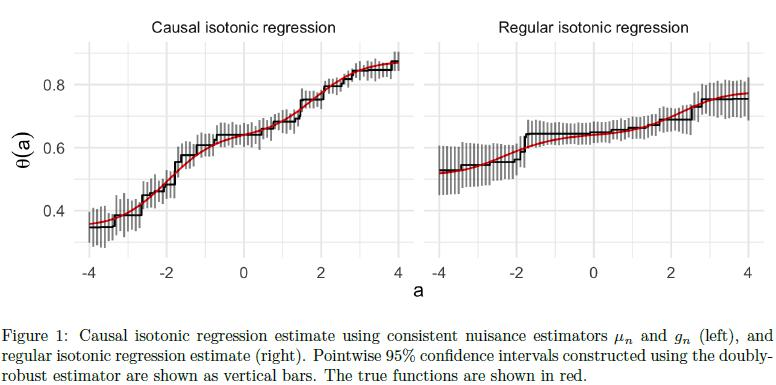
\includegraphics[width=8cm]{Causal Isotonic Regression/CIRS501}

\end{frame}

%%%%%%%%%%%%%%%%%%%%%%%%%%%%%%%%%%%%%%%%%%%%%%%%%% p.15

\begin{frame}{Simulation Results}

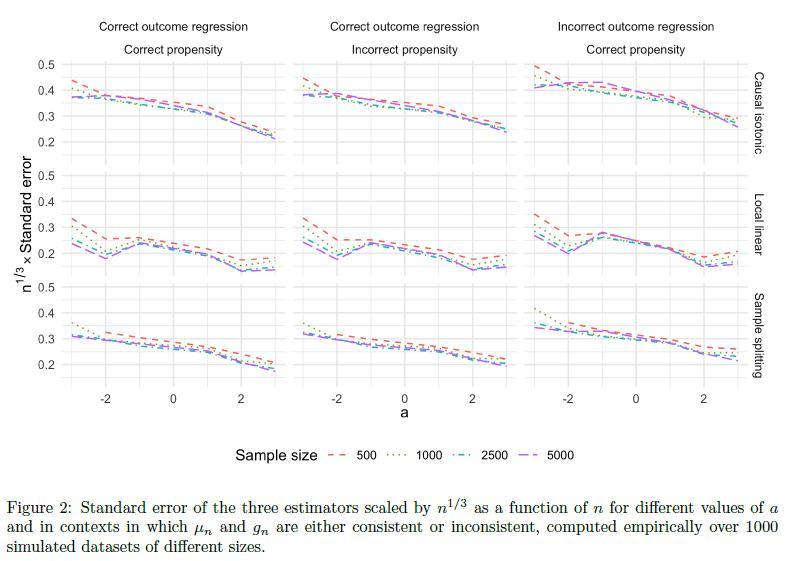
\includegraphics[width=11cm]{Causal Isotonic Regression/CIRS502}

\end{frame}

%%%%%%%%%%%%%%%%%%%%%%%%%%%%%%%%%%%%%%%%%%%%%%%%%% p.16

\begin{frame}{Simulation Results}

\begin{block}{Standard error}
	\begin{enumerate}
	\item	The standard error of the local linear estimator is smaller than that of $\theta_n$, is expected due to the fast rate of convergence.
	\item	The standard deviation of the local linear estimator appears to decrease faster than $n^{-1/3}$.
	\item	Inconsistent estimation of the propensity has little impact on the standard errors of any of the estimators but inconsistent estimation of the outcome regression not.
	\end{enumerate}
\end{block}

\end{frame}

%%%%%%%%%%%%%%%%%%%%%%%%%%%%%%%%%%%%%%%%%%%%%%%%%% p.17

\begin{frame}{Simulation Results}

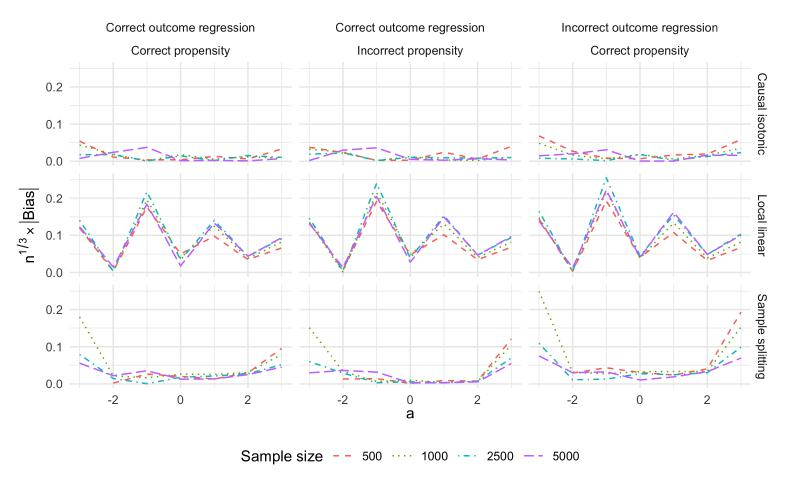
\includegraphics[width=11cm]{Causal Isotonic Regression/CIRS503}

\end{frame}

%%%%%%%%%%%%%%%%%%%%%%%%%%%%%%%%%%%%%%%%%%%%%%%%%% p.18

\begin{frame}{Simulation Results}

\begin{block}{Absolute bias}
	\begin{enumerate}
	\item	The estimator of $\theta_n$ has smaller absolute bias than the local linear estimator, and its absolute bias decreases faster than $n^{-1/3}$.
	\item	The absolute bias of the local linear estimator depends strongly on $a$, and in particular is largest where the second derivative of $\theta_0$ is larger in absolute value.
	\item	The sample splitting estimator has larger absolute bias than $\theta_n$ since it inherits the bias of $\theta_{n/m}$. The bias is large for values of a in the tails of the marginal distribution of A.
	\end{enumerate}
\end{block}

\end{frame}

%%%%%%%%%%%%%%%%%%%%%%%%%%%%%%%%%%%%%%%%%%%%%%%%%% p.19

\begin{frame}{Simulation Results}

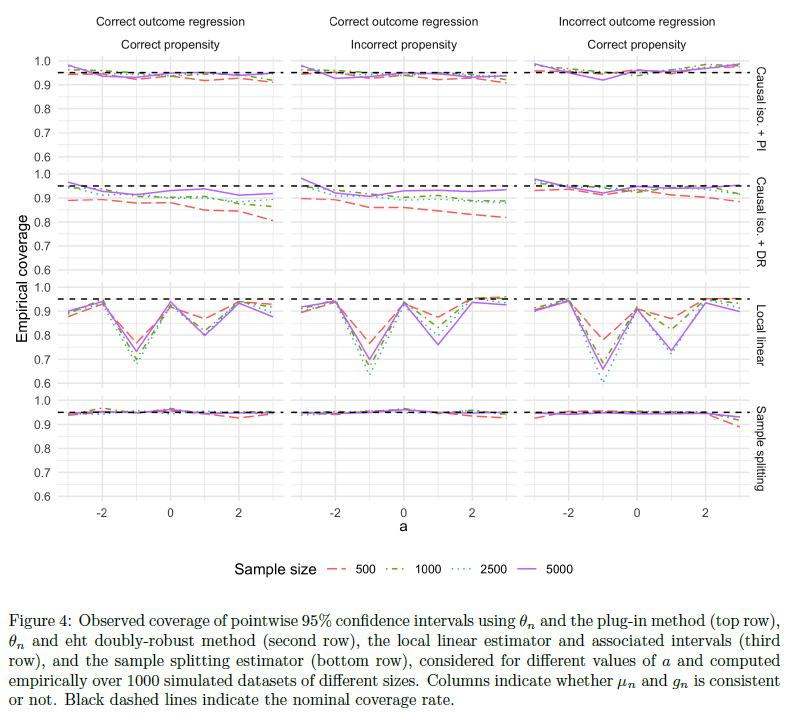
\includegraphics[width=11cm]{Causal Isotonic Regression/CIRS504}

\end{frame}

%%%%%%%%%%%%%%%%%%%%%%%%%%%%%%%%%%%%%%%%%%%%%%%%%% p.20

\begin{frame}{Simulation Results}

\begin{block}{Coverage of pointwise 95$\%$ confidence intervals}
	\begin{enumerate}
	\item	Both plug-in and doubly-robust estimator intervals centered around $\theta_n$, the coverage improves as n grows.
	\item	Under correct specification of outcome and propensity regression models, the plug-in method attains close to nominal coverage. When the propensity estimator is inconsistent, the plug-in method still performs well in this case. When $\mu_n$ is consistent, the plug-in method is very conservative for positive values of a.
	\item	The doubly-robust method attains close to nominal coverage for large samples as one of $g_n$ or $\mu_n$ is consistent.
	\item	The local linear estimator has poor coverage for values of $a$ where the bias of the estimator is large.
	\item Sample-splitting method performs excellent except perhaps the value of a in the tails when $n$ is small or moderate.
	\end{enumerate}
\end{block}

\end{frame}

%%%%%%%%%%%%%%%%%%%%%%%%%%%%%%%%%%%%%%%%%%%%%%%%%% p.21

\begin{frame}{Simulation Results}

	A simulation study is conducted to illustrate the performance of the proposed procedures when machine learning techniques are used to construct $\mu_n$ and $g_n$.

\begin{block}{Estimator under settings}
	Consider the estimator $\theta^{\circ}_n$ obtained via cross-fitting (mentioned in section 3.7).
	\begin{enumerate}
	\item If $\mu_n$ is consistent, then use Super Learner (van der Laan et al. 2017)
	\item If $g_n$ is consistent, then used the method proposed by Diaz and van der Laan(2011) with covariate vector $(W_1,W_2,W_3,W_4)$.
	\item If $\mu_n$ or $g_n$ is inconsistent, then omit covariates $W_1$ and $W_2$.
	\end{enumerate}
\end{block}

\end{frame}

%%%%%%%%%%%%%%%%%%%%%%%%%%%%%%%%%%%%%%%%%%%%%%%%%% p.22

\begin{frame}{Simulation Results}

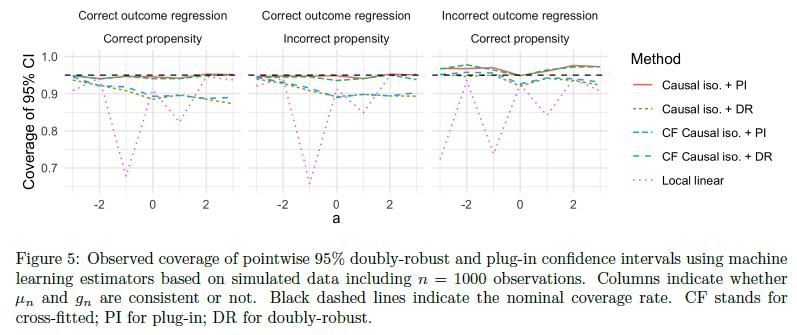
\includegraphics[width=12cm]{Causal Isotonic Regression/CIRS505}

\end{frame}

%%%%%%%%%%%%%%%%%%%%%%%%%%%%%%%%%%%%%%%%%%%%%%%%%% p.23

\begin{frame}{Simulation Results}

\begin{block}{Coverage of 95$\%$ of confident intervals}
	\begin{enumerate}
	\item The plug-in method performs well which achieve very close to nominal coverage under both consistent settings, even propensity is inconsistently estimated.
	\item The doubly-robust method is anti-conservative under both inconsistent settings and also when the propensity is inconsistently estimated. Good coverage rates are also achieved when the outcome regression is inconsistently estimated.
	\item Cross fitting has little impact on coverage.
	\end{enumerate}
\end{block}

\end{frame}

%%%%%%%%%%%%%%%%%%%%%%%%%%%%%%%%%%%%%%%%%%%%%%%%%% p.24

\begin{frame}{Simulation Results}

\begin{block}{Conclusion of results}
	\begin{enumerate}
	\item For plug-in method, under the inconsistent estimation of any nuisance function, the scale parameter is biased and its variance decreases relatively quickly with sample size by the simple empirical average of estimated functions.
	\item For doubly-robust method, the scale parameter is asymptotically unbiased but its variance decreases much slower with sample size.
	\end{enumerate}
\end{block}

\end{frame}

\section{Body mass index and T-cell response in human immunodeficiency virus vaccine studies}

\begin{frame}{Literature Review on BMI and cells response}
Some previous scientific literature indicates that
\begin{enumerate}
	\item BMI is inversely associated with immune responses to vaccination

	\item higher BMI might lead to impaired	immune responses

	\item obesity reduced hepatitis B immune responses through leptin-induced systemic and B cell intrinsic inflammation, impaired T cell responses
\end{enumerate}
\textbf{AIM:} assess the covariate-adjusted relationship between BMI and CD4+ T-cell responses using data from a collection of clinical trials of candidate HIV vaccines
\end{frame}

\begin{frame}{Comment on previous literature}
\begin{enumerate}
	\item Jin et al. (2015): low BMI participants had a statistically significantly greater response rate than high
	BMI participants by using Fisher's exact test.\\
	\textit{Comment:} Marginal comparison can be misleading due to existence of confounders such as age and sex.

	\item Jin
	et al. (2015): logistic regression of the binary CD4+ responses against sex, age,
	BMI (not discretized), vaccination dose and number of vaccinations.\\
	\textit{Comment:} adjusted odds ratio has a formal causal interpretation only under strong parametric
	assumptions.
\end{enumerate}
Comparetively, the method proposed in this paper can identify the covariate-adjusted dose-response function
$\theta_0$ with the causal dose-response curve without making parametric assumptions.
\end{frame}

\begin{frame}{Argument in Causal inference}
Some researchers suggest that causal model should always be tied to hypothetical randomized experiments. However, randominzed experiments are commonly not practical. For example,
\begin{enumerate}
	\item Not ethical to force someone to smoke or not to smoke
	\item \textbf{Impossible} to assign the BMI to the participants randomly.
\end{enumerate}
one may think it is not appropriate to interpret the G-computed regression function $\theta_0(a)$ in causal manner. \\
However, it provides a meaningful summary of the relationship between BMI and immune
response accounting for measured potential confounders.
\end{frame}

\begin{frame}{Result}
	\begin{center}
		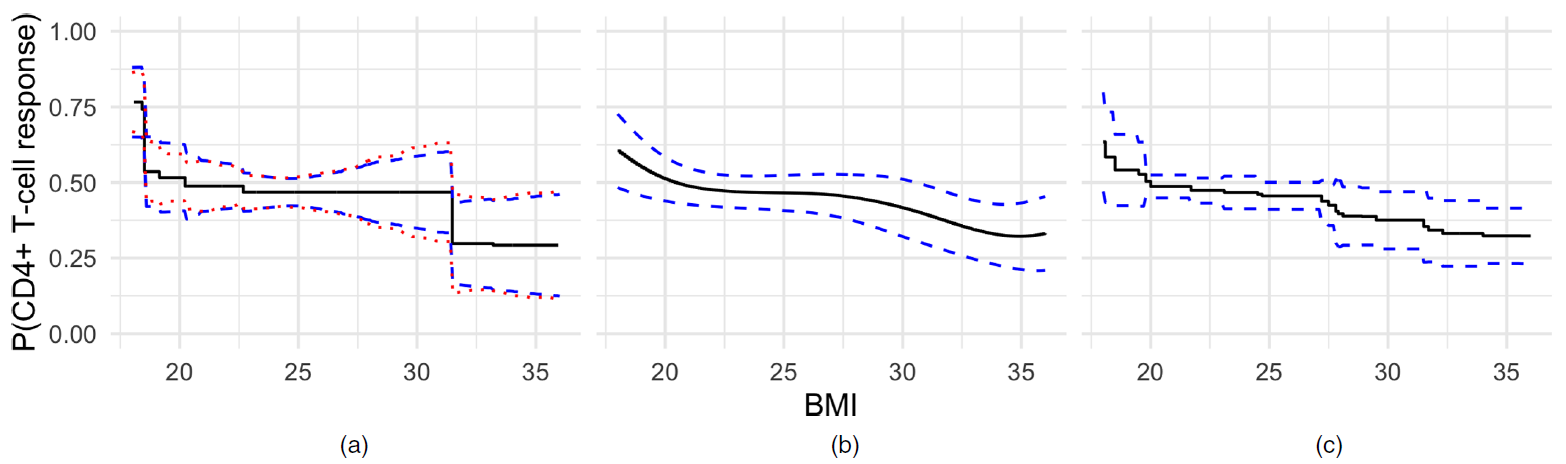
\includegraphics[width=120mm,height=40mm]{Causal Isotonic Regression/Fig_Sec6}
	\end{center}
The graph refer to the estimated probabilities of CD4+ T-cell response and 95\% pointwise confidence intervals as a function of BMI, adjusted for sex, age, number of vaccinations received, vaccine dose and study with
\begin{enumerate}
	\item Estimator proposed here
	\item Local linear estimator of Kennedy et al. (2017)
	\item Sample splitting version of our estimator with $m=5$ splits
\end{enumerate}
\end{frame}

\section{Concluding remarks}
\begin{frame}{Furture direction}
	\begin{enumerate}
		\item Inference on a monotone causal dose-response curve when outcome data are only observed subject to potential coarsening, such as censoring, truncation or
		missingness

		\item Develop tests of the monotonicity assumption.

		\item Develop methods for uniform inference.

		\item Inferential methods that do not require estimation of additional nuisance parameters or sample splitting
	\end{enumerate}
\end{frame}

\begin{frame}{Comparison between methods}
There is some tradeoff between local linear smoothing and monotonicity-based methods.
\begin{enumerate}
	\item Convergence rate of regression estimator:\\
	faster for local linear regression estimator; $n^{-2/5}$ VS $n^{-1/3}$ for monotonicity based method.

	\item Local linear smoothing: Limit distribution
	involves an asymptotic bias term depending on the second derivative of the true function,
	so confidence intervals based on optimally chosen tuning parameters provide asymptotically
	correct coverage only for a smoothed parameter rather than the true parameter of interest.

	\item Monotonicity based: Do not require choosing a tuning parameter, are invariant to strictly
	increasing transformations of the exposure and their limit theory does not include any asymptotic
	bias.
\end{enumerate}
\end{frame}

\end{document}
